%
% File: outline.tex
% Author: Oliver J. H. Feighan
% Description: Thesis outline
% Thesis outline
%
%\let\textcircled=\pgftextcircled
\chapter{Introduction}
\label{chap:intro}

\initial{P}hotosynthesis is the bedrock of life on this planet. It is often the 
first step in the food chain, establishing ecosystems from a near unlimited source 
of sunlight. The earliest evidence of photosynthetic organisms was formed around
3.5 billion years ago \cite{Blankenship2010}. One of the most studied organims are
purple bacteria, \cite{Cogdell2021}. These organisms use light harvesting complexes 
(LHCs) to absorb and stabilise energy from light which is eventually transferred 
to reaction centres \cite{Klamt2008}. The mechanism for creating adenosine triphosphate
occurs at these reaction centres using the photonic energy for charge transfer.
These complexes are extremely efficient, with the LHC found in purple bacteria being
around 95\% efficient at transferring the electronic energy to charge separation \cite{Tretiak2000}.

Many types of complexes exist, differing by the type of chlorophyll pigments as 
well as structural features. Most often these complexes are formed of repeated units.
For example the LH2 complex found in \emph{acidophilus} is formed of a trimer unit
with two bacterial chlorophyll \emph{a} (BChla) chromophore in close proximity, 
aligned parallel along the porphyrin plane, with a third chromophore perpendicular
and further apart (shown in figure \ref{fig:LH2_subunit}). This unit is then repeated
to form a circular structure, with anywhere between an 8-10 fold symmetry depending 
on the environment in which the bacteria grow (see figure \ref{fig:LH2_rings}). 
It is thought that the efficiency of these LHCs is mostly due to these structures,
and the conformations of the chromophores.

\begin{figure}
	\centering 
	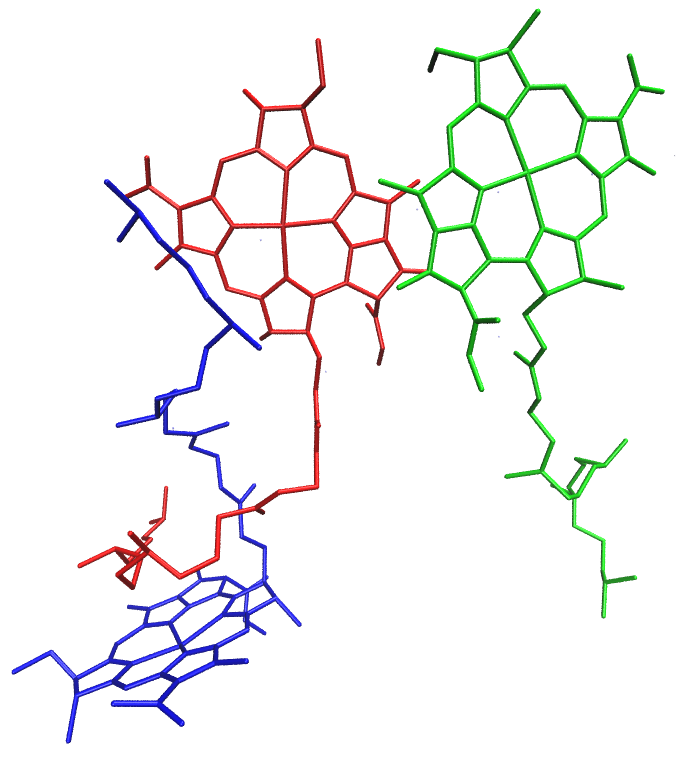
\includegraphics[scale=0.3]{chapters/1_introduction/subunit.png}
	\label{fig:LH2_subunit}
	\caption{The trimer unit found in LH2, coloured by ring type (red and green
	for B850a and B850b, blue for B800).}
\end{figure}

\begin{figure}
	\centering 
	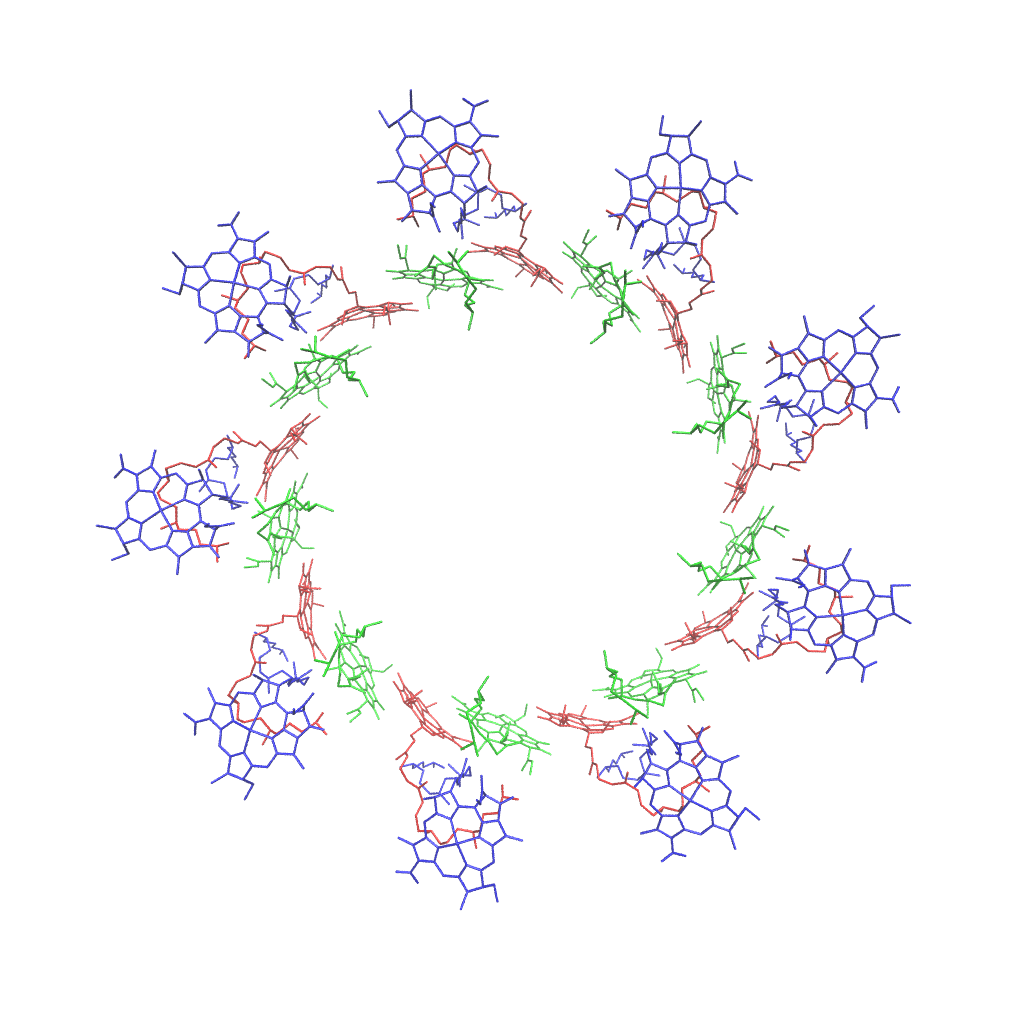
\includegraphics[scale=0.3]{chapters/1_introduction/ring_assign.png}
	\label{fig:LH2_rings}
	\caption{Aggregate units found in LH2, coloured by ring type (red and green
	for B850a and B850b, blue for B800). This particular structure has a 9-fold
	symmetry, giving the circular ring structures.}
\end{figure}

Detailed computational study of these structures has been possible since the first
crystal structures were elucidated, and has produced a wealth of analysis from investigations
of the properties of these complexes that could only be calculated from computational
methods. Most recently these include the effects of non-covalent bonding on the 
chlorophyll pigments, etc. These studies show that the effects of the protein occur
on the atomistic level as well as on the order of the whole protein structure.

A physical model of LHCs can be given by constructing a Hamiltonian for the system,
similar to any other electronic structure problem. However due to the size of the
complexes it is usually necessary to reduce the number of degrees of freedom in
these Hamiltonians. For LH2, the chlorophyll system alone contains 3780 atoms, with
an additional ~6000 atoms for the entire scaffold. Including a membrane and explicit
solvent can quickly lead to system sizes in the region of 300,000 atoms.

Usual electronic structure methods that describe molecular excited states (e.g. 
DFT) are not tenable for LHCs. Instead a Frenkel-Davydov model is more appropriate
due to the weak coupling, and this model recaptures the delocalisation of excited
states over pigment sites. This model constructs the Hamiltonian from intra-site 
energies and inter-site interactions, reducing the degrees of freedom of the Hamiltonian
from the entire state to just single chromophores. A more formal description is 
given in the next chapter.

The Frenkel exciton Hamiltonian can either be constructed from static parameters,
fit to experimental data or calculated theoretical values, or as functions of LHC 
geometry and/or time. To recover a truly atomistic treatment of LHCs it is necessary 
to take the second approach, which if looking at dynamic properties can be far more
expensive to calculate as Hamiltonians are required for every frame in a time series 
of LHC geometries, explicitly treating the geometry variations. This also comes 
with the caveat that methods used to construct the exciton Hamiltonian have to be
highly accurate, as geometry variations are usually very small, although this is
also used as a reason take a more averaging approach.

Often LHC models fall into a similar pattern. Electronic structure calculations
are used to produce excited state properties for individual sites, which in turn 
are used to construct Frenkel exciton Hamiltonians, ultimately giving the excited 
states of the whole LHC. It is obvious then where the model design choicesa are. 
First is which electronic structure and response method to use to calculate intra-
site properties, and second how to use these properties to construct the exciton 
Hamiltonian. The decisions on these choices is highly dependent on the level of 
detail required for the exciton system (atomistic or coarse grain), and the volume
of unique Hamiltonians required (how many frames of molecular dynamics are used).
For a coarse-grain model, where the full geometry of the chlorophyll system is not
important, then a more approximate method could be used.

For a truly atomistic approach often density functional theory (DFT) and linear 
response methods (time-dependent DFT or TD-DFT) are used to calculate single site
properties. Due to the size of chlorophyll molecules, using high level methods such 
as coupled cluster and EOM-CCSD would not be reasonable. Even with TD-DFT methods
only a limited number of explicit Hamiltonians could be constructed before the cost 
is too high. If a large number of LHC geometries need to be calculated then further
approximations are necessary.

This trade-off between computational expense and fine-grain accuracy is the main
issue in designing physical models for LHCs. Often it is found that while coarse-
grain models are good enough, smaller details are lost when not using models where
the electronic structure and response calculations necessary are too expensive. 
Some solutions to this problem are offered in the literature which are discussed
below, however each have limitations. These limitations sketch out the potential
for a new kind of LHC model, which is described at the end of this chapter.

\section{Efficient Response Methods}
\label{sec:efficient_response_methods}

The most obvious solution to this problem is to make the electronic structure and
response calculations more efficient. This is often at the expense of accuracy.
Many recent studies use tight binding methods such as TD-DFTB or ZINDO to calculate
response properties. These methods can include environmental effects (such as continuous
solvent models or point charge embedding), and are implemented in a wide range of
electronic structure packages. However they have been argued to be limited by their
accuracy, making them not reliable for the complex \Qy transition important to many
LHCs. Often as well these methods are black-box and not easy to reparameterise due
to the complex interdependecy of parameters. 

This issue has been addressed by the xTB methods developed by Grimme \emph{et al.}.
A more in-depth discussion of these methods is given in the next chapter. The sTDA-xTB
method is a direct solution to the problem set out above, aiming to calculate accurate
transition properties with greater efficiency than the TD-DFT workhorse. To fully
appreciate how this is done, an outline and discussion of this method is given below.

\subsection{sTDA-xTB}
\label{subsec:stda_xtb}
sTDA-xTB ("simplified Tann-Dancoff Approximation - eXtended Tight Binding") is another
method in the family of xTB methods developed by the Grimme group, and is parameterised
for transition properties \cite{Grimme2016}. The accuracy in calculating transition energies with this
method is very good, with the error compared to high-level method, such as SCS-CC2,
being around 0.3 - 0.5 eV.

Similar to other xTB methods, sTDA-xTB is based on tight-binding electronic structure
that uses empirically fitted parameters and a minimal basis set. It was trained 
on a set of highly accurate coupled cluster and density functional theory excitation 
energies, as well as atomic partial charges for inter-electronic interactions.

Unlike other xTB methods, coefficients in the basis set for sTDA-xTB are dependent
on coordination number of the atom centres. This makes basis functions far more 
flexible, which would with fixed basis function could only be achieved by using 
diffuse or additional orbitals in the basis set. It also uses two sets of parameterized 
basis sets - a smaller valence basis set (VBS) and an extended basis set (XBS).
Whilst this reduces the cost of having larger basis sets, it makes calculating the
gradient of transition properties much more difficult.

The two basis sets are used to construct formally similar Fock matrix elements,
although in practice they use different global parameters. The core Hamiltonian
is similar to other DFTB methods that use a self-consistent charge (SCC) method 
to obtain molecular orbital (MO) coefficients. It is given by

\begin{equation}
\bra{\psi_\mu} H^{\text{EHT, sTDA-xTB}} \ket{\psi_\mu}= \frac{1}{2} \left(k^l_\mu k^{l'}_\nu\right) \frac{1}{2} \left(h^l_\mu h^{l'}_\nu\right) S_{\mu\nu} - k_T \bra{\psi_\mu}\hat{T}\ket{\psi_\nu}
\end{equation}
%
where $\mu,\nu,l,l'$ are orbital and shell indices, $k^l_\mu$ are shell-wise 
H{\"u}ckel parameters, $h$ are effective atomic-orbital energy levels, $S_{\mu\nu}$
is the overlap of orbitals $\mu$ and $\nu$, $k_T$ is a global constant and $\hat{T}$
is the kinetic energy operator. The charges used in the inter-electronic repulsion 
function are given by charge model 5 (CM5) \cite{Marenich2012} charges for the XBS
Fock matrix. These are calculated using Mulliken charges obtained from diagonalising
the Fock matrix with the VBS. The charges for the initial VBS Fock matrix are based
on Gasteiger charges \cite{Gasteiger1978}, modified by the parameterised
electronegativities of atoms in the system.

The whole process for determining molecular orbitals can be summarized as:
\begin{enumerate}
	\item Calculate modified Gasteiger charges for the first initial guess
	\item Diagonalise Fock matrix in the VBS to get the first set of Mulliken charges
	\item Compute CM5 charges
	\item Diagonalise Fock matrix in the VBS again for final set of Mulliken charges.
	\item Recalculate CM5 charges with this final set, and diagonalize the Fock matrix in the XBS. 
	\item The molecular orbital coefficients from this are then fed to the response theory.
\end{enumerate}

The response theory for this method is based on previous work in the Grimme group
on the simplified Tamm-Dancoff Approximation \cite{Grimme2013}. There are several
approximations made between full linear response theory and the sTDA method. First
is the Tamm-Danncoff approximation, where some transition characters are ignored. 
The second approximation is to use a Mataga-Nishimoto-Ohno-Klopman (MNOK) method 
to calculate 2 electron integrals instead of explicitly calculating them.

Transition charges are used to calculate these MNOK integrals. These charges $q^A_{nm}$
(centred on atom $A$ and associated with the transition $ n \rightarrow m$) are
computed using a Löwdin population analysis

\begin{equation}
q_{nm}^A = \sum_{\mu \in A} C^\prime_{\mu n} C^\prime_{\mu m}
\end{equation}

where the transformed coefficients $C^\prime_{\mu n}$ are given by orthogonalising
the original MO coefficients $\textbf{C}$

\begin{equation}
\textbf{C}^\prime = \textbf{S}^{\frac{1}{2}} \textbf{C}
\end{equation}

and $\mu$ is an index that runs over the atomic orbitals (AO). The MO coefficients
are the solution of diagonalising the Fock matrix, similar to equation \ref{eq:roothaan_hall}.

The approximations to full 2 electron integrals are given by charge-charge interaction
damped by the MNOK\cite{Nishimoto1957}\cite{Ohno1964}\cite{Klopman1964} functions.
For exchange and coloumb type integrals, difference exponents are used, along with
an additional free parameter to recover the amount of Fock exchange mixing in
the original matrix element equation. These will be discussed in more detail in
chapter \ref{chap:chl_xtb}, as they are a crucial part of designing a new response 
method for chlorophyll systems.

Lastly the single particle excited space used to construct the $\mathbf{A}$ matrix
is truncated more than that of normal TD-DFT. This reduces the number of elements
that need to be calculated, reducING the time taken for diagonalisation whilst also
capturing a broad enough spectrum of excitation energies. 

The sTDA-xTB method is reported as having excellent accuracy against benchmarked
data, and has been used to generate absorption spectra and other properties for 
large systems. At first glance, it would seem that this method would solve the issue
of calculating many Frenkel exciton systems. However this is not entirely given 
by the data so far. Much of the data expressing sTDA-xTB accuracy has been performed 
on a range of systems, and does not concern smaller variations of a single system. 
The latter is more important for LHCs, as the variations in chlorophyll geometries
that cause variations in the exciton system are relatively small. Without any indication
on how accurate sTDA-xTB is for a range of conformers it is difficult to say whether
it would be better than previously used tight-binding methods. It may be better 
to start from methods that do have accurate correlations with system geometries, 
such as TD-DFT, and work from this to retain accuracy. This is explored in the next
section on statistical method based on high-level data to generate new values for
exciton models.

\section{Statistical Methods}
\label{sec:stats_methods}

Making approximations in constructing the exciton framework is an alternative option
to response method approximations. One of the simplest ways of doing this is by 
using static parameters fit from experimental or calculated data. These are referred
to static as they do not vary between frames in a time series of LHC geometries. 
Using these static Hamiltonians negates any variation in intra-chromophore or protein
scaffold geometry, but can still produce good predictions of physical phenomena.

If using a long timescale, where the full conformation space is well sampled, exciton
Hamiltonians can be constructed from distributions of chromophore response properties
(i.e. excitation energies and transition densities). These properties would be distributed
along a normal distribution when taken from a set of uncorrelated structures. The
mean and standard deviations can then be used to define a distribution function 
which can be limitlessly sampled to construct Hamiltonians without the need for 
explicit calculations on structures. The Hamiltonians could utilise functions that 
take into account inter-chromophore geometries, for example by calculating coupling
values from a distribution function of transition dipole magnitudes, or use distributions
for all elements of the Hamiltonian matrix.

These methods are mostly based on static parameters, such as the mean and standard
deviation or the Hamiltonian elements themselves, and are not functions of time.
This means they would be ill-suited for dynamic studies where structures at different
times are correlated. However recently machine-learning methods has been reported
that would give time-dependent Hamiltonians still without the need for explicit
calculations.

\subsection{Machine-Learning For Exciton Models}
\label{subsec:machine_learning} 

Machine-learning models have been used in many areas of computational chemistry,
especially in areas where both large amounts data and numerical metrics make it 
easy to train these methods. At their heart, these methods are similar to the static
statistical methods that have already been used for LH2 exciton systems, as they
rely on parameters fit to high level data. However these new models use machine-
learning techniques to incorporate atomic geometry information, making them time
dependent.

In 2016 H\"{a}se \emph{et al.} reported on a multi-perceptron (also referred to
as a neural network (NN)) model that predicts the \Qy transition for chlorophyll
molecules. Using this model, as well as fitted parameters for the exciton coupling,
it was possible to calculate exciton population dynamics, as well as spectral densities
for chlorophyll sites in the FMO light harvesting complex. Similar to other models
a Coloumb matrix is used as descriptor of the chlorophyll systems, defined as 

\begin{equation}
	M_{AB} = 
	  \begin{cases}
		\frac{1}{2} Z^{2.4} \text{ for } A = B\\
		\frac{Z_A Z_B}{\left\lvert \mathbf{R}_A - \mathbf{R}_B\right\rvert} \text{ for } A \neq B
	  \end{cases}
\end{equation}
%
where $Z_A$ is some measure of the atomic charge on atom $A$, and $R_A$ is the position
vector. It can be seen that the off-diagonal elements are simply the Coloumbic interactions,
and diagonal elements are a polynomial of the atomic charges. This descriptor is
popular due to the similarity in information that an electronic structure calculation
would start from, namely the positions and nuclear charges of atoms.

This matrix is used as an input for a neural network made from perceptrons structured
into layers. Briefly, a neural network is a series of matrix multiplications applied
to input data that overall acts as a non-linear function. These multiplications 
are organised into steps, referred to as layers, with the first and last called 
input and output layers and any steps in-between referred to as "hidden" layers in-between.

\begin{figure}
	\centering
	\begin{neuralnetwork}[height=4]
        \inputlayer[count=3, bias=true, title=Input\\layer]
        \hiddenlayer[count=4, bias=false, title=Hidden\\layer 1] \linklayers
        \hiddenlayer[count=3, bias=false, title=Hidden\\layer 2] \linklayers
        \outputlayer[count=2, title=Output\\layer] \linklayers
	\end{neuralnetwork}
	\label{fig:neural_network}
	\caption{Simplified schematic of a neural network showing how input values,
	such as the Coloumb matrix, can be used to generate outputs by several matrix
	multiplications and activation functions (represented by the arrows). The values
	in the output layer for models discussed in the text would be \Qy transition
	energies or atom centered transition charges.}
\end{figure}

A layer is a distinct vector of values. For example, flattening the Coloumb matrix
into a 1D vector gives the input layer, and the \Qy transition energy is a the output 
vector (of 1 element). A vector at layer $n$, is multiplied with a coefficient matrix 
$c$ to give the next layer

\begin{equation}
	\mathbf{V}_{n+1} = \mathbf{c}_n \mathbf{V}_n	
\end{equation}
%
where the coefficient matrices $\mathbf{c}_n$ are fitted to give the smallest deviations
of the output layer against target data (i.e. error in predicted \Qy energies in 
this case). Often additional functions are used to modify these values, such as
sinusoidal, sigmoid, linear ($\tilde{V}_{n+1}=m V_{n+1}$) or rectified linear unit 
($\tilde{V}_{n+1}=\text{max}\left(0, m V_{n+1} \right)$) functions. In this way they 
are conceptually similar to biological neurons which take in electrical signals 
and through some mechanism are can be activated to send out a different signal. 
The coefficient matrices $\mathbf{c}_n$, and any other parameters in the activation
functions, are fit by a back-propagation method which also uses parameters - these 
are referred to as hyper-parameters and can be optimised using a systematic grid-search
to learn the best coefficient matrix. Other considerations such as over-fitting 
also need to be taken into account. The brief explanation of NNs here is fairly 
simplistic, and creating these models takes in-depth knowledge and experience to
achieve good results.

This model predicted \Qy transition energies with around a 0.3 meV error for all
of the 8 sites in the FMO complex. This is exceptionally accurate, supporting the
idea that atomic positions and nuclear charges contain all the information necessary
to predict transition energies. It is noted in this work that the Nitrogen root
mean squared deviations (RSME) correlates well with excited state properties. Exciton
properties, such as the time series of exciton populations, were also well reproduced
using these \Qy energies, although the coupling parameters were taken from other
fits and not from a NN method.

Another method, developed by Farahvash \emph{et al.}, utilised both neural networks
and kernel ridge regression (KRR) to predict both site energies as well as exciton 
coupling parameters, giving a completely time dependent exciton Hamiltonian. KRR
is another machine-learning method, that can be understood as two processes. First
is the ridge regression, which is similar to a linear regression model but with
an additional factor to account for co-linear relationships between inputs. Regression
models are multivariate linear models that follow the form

\begin{equation}
	f^\prime\left(\mathbf{X}\right) = \mathbf{X} \mathbf{\beta}
\end{equation}
%
where $f^\prime\left(\mathbf{X}\right)$ are the predicted values of some metrics $f\left(\mathbf{X}\right)$ 
(i.e. \Qy energy or exciton coupling value), $\mathbf{X}$ is the matrix of information
used to predict the value $f$ (i.e. flattened Coloumb matrix, referred to as the feature
matrix) and $\beta$ is a set of fitted coefficients that minimise the value $\left\lvert f^\prime \left( \mathbf{x}\right) - f \left(\mathbf{x}\right)\right\rvert$.
The matrix $\mathbf{\beta}$ can be found by minimising the square of this value, 
a method known as the least-squares method, however this can lead to expensive terms 
when calculating the inner product of the feature matrix. Here the "kernel trick" 
is used to make these terms easier to calculate. This rearranges the minimisation 
of regression coefficients so that the inner products are not required, but requires 
a new function that compares the similarity of features. Glossing over derivation
details, the function $f^\prime$ becomes

\begin{equation}
	f_{\text{KRR}}^\prime = \sum^{N_x}_j \beta_j k\left(\mathbf{x}, x_j\right)
\end{equation}
%
where the $N_x$ is the size of the feature vector $\mathbf{x}$ (which is the linear
model is stacked to form the matrix $\mathbf{X}$), and $k$ is the kernel function.
Often this is a gaussian function of the feature vector

\begin{equation}
	k\left(\mathbf{x}, x_j\right) = \text{exp}\left(\frac{-\left(\mathbf{x}-x_j\right)^2}{2\sigma^2}\right)
\end{equation}
%
where $\sigma$ is a fitted parameter. Again these parameters are optimised by a 
systematic search through values, similar to the grid search referenced before.

A KRR model was developed for both the excitation energies and exciton coupling 
parameters. However it was found that a NN model predicted exciton couplings with
greater accuracy, which was attributed to the more complex conformational space.
This NN model calculated atomic centered transition charges which were then used
to calculate coupling elements with small error against higher level methods.

These machine-learning models show that it is possible to generate time (and geometry)
dependent functions that give either transition properties needed to construct exciton
Hamiltonians or the full Hamiltonians themselves. However there are some unaddressed
issues. In contrast to the sTDA-xTB method, these machine learning models do not 
use any formalism that treats the electronic structure explicitly. This makes it
difficult to include any other affects, such as continuous solvent models or point
charge embedding, that are often used in LHC quantum mechanics / molecular mechanics 
(QM/MM) models. Some models do use QM/MM methods to generate training data, but 
this would only lead to pigeonholing the optimised model to the QM/MM system used.
This is the main scientific issue with this approach. There are some practical
considerations as well, such as the requirement of in-depth knowledge of machine-learning 
methods to retrain models, as well as the cost of generating large amounts of high
level training data.

\section{GPU Acceleration}
\label{sec:gpu_acceleration}

An alternative approach to this problem would be to accelerate the TD-DFT calculations.
This approach has been used previously to construct Frenkel exciton Hamiltonians
for the LH2 complex based on $\omega\text{PBEh}$/6-31G TD-DFT calculations. Graphical 
processing units (GPUs) can partition a limited number of basic operations over 
a massive number of parallel components, which can be exploited to parallelise expensive 
electron integrals. These are often the bottleneck for most TD-DFT calculations.
This approach does not require any parameter optimisation or new formalism but does
require appropriate hardware (GPU cards) and programs that can partition on GPUs
correctly, however this is a common feature on high performance computers. GPU-acceleration
has been used in many other computational chemistry studies, and is a popular way 
of drastically increasing system sizes while keeping computing time down.

This model was benchmarked against TD-DFT calculations on a hexamer of bacterial
chlorophyll \emph{a} molecules from LH2, and had an average error of 0.008 eV. Comparisons
to absorption spectra predicted by full TD-DFT and the exciton model were also favourable, 
as were predictions of dynamic properties of the exciton system.

Whilst computing the electron integral terms are far less time intensive, storing
these values is a major issue. This is due to the lightweight memory restrictions
on GPU cards, and even makes recalculation of some integrals more efficient than
storage. This means that a larger basis sets may be too expensive to utilise. It
could be argued that this lack of high level detail would make a niche method, one
which uses more approximate response methods but is better at reproducing high level
data, more suitable for some studies. This would lead back to using machine-learning
methods, however this work proposes a novel approach outlined below.

\section{Combining Approaches}
\label{sec:possible_novel_methods}

The underlying issue of LHC models is clear - the systems are too large to explicitly
calculate all transition properties required by high level methods. Making well 
chosen approximations has found success in solving parts of this issue, but often
at with compromises. The sTDA-xTB method (and other tight-binding methods) are efficient
but possibly not accurate enough to give meaningful results. Machine-learning methods
are accurate and efficient but not extendable, use large amounts of expensive high
level training data, and require a good understanding of machine-learning methods.
Accelerating calculations with hardware can also be used but may still come up against
memory issues, however inevitable progress in high performance machines will fix 
this eventually.

These shortcomings sketch out the need for a method that is efficient, accurate,
extendable, memory light and easy to reproduce. Combining approaches would be expected
to keep benefits whilst addressing shortcomings. The tight-binding approaches show
that even a low level electronic structure is enough to capture the main features
required for accurate transition properties. The machine-learning models show that
is using a high degree of specificity can train methods to be extremely accurate.
This forms the main thesis of this work - that there is merit in designing a method
for light harvesting models that combines these benefits. The results presented in 
chapters \ref{chap:dscf} and \ref{chap:chl_xtb} test this idea, and a discussion
of the results propose reasons why these methods may or may not solve the shortcomings
outlined above. Applications of these methods to LHC properties are also explored
in chapters \ref{chap:excitons} and \ref{chap:LH2} to further explore whether the
novel features of this combinatorial approach can elucidate new explanations of
LHC phenomena.